\section{Precision of Indoor Location}\label{sec:estimoteprecision}
Another core part of our system is indoor location. 
For the ``point-to-select'' part of our system to work as intended, 
we need high indoor precision. 
In \Cref{sec:design:indoor-positioning} we mentioned that Estimote claims the accuracy to be \num{0.5}-\num{1} meters.
In this section we test if that is actually the case, 
or even if we can achieve better results than that. 
This section will contain some of the measurements from our tests. 
All of the measurements can be found in \Cref{app:estimotetestresults}

We test this by comparing the position we get from the application, \ie from the Estimote beacons,
to the actual position we have measured in the room using a measuring tape.
We test it with the \num{4} settings from \Cref{table:rooms}.

\begin{table}
  \centering
  \begin{tabular}{l| l c c c}
    Name & Size in meters & \# of Beacons & \# of Tests & \# of WiFi Access Points\\ \hline
    Room 1 & $5 \times 5$ & 4 & 8 & 19 \\
    Room 2 & $8 \times 8$ & 4 & 7 & 19 \\
    Room 3 & $17.9 \times 17.9$ & 4 & 3 & 3\\
    Room 4 & $4.9 \times 9.95$ & 4/8 & 33 & 20 
  \end{tabular}
  \caption{Room settings}
  \label{table:rooms}
\end{table}

We tested in different settings to measure if, and how much, 
the size of the room matters in terms of accuracy. 
We decided to test outside in an area where there were none or few WiFi signals,
as WiFi shares the same same radio frequency as BLE (\SI{2.4}{\GHz}). 
We have performed tests both with and without movement. 
The same person performed all the movement tests. 

\subsection{Setup}\label{sec:setup}
Room 1 and Room 2 were setup in an auditorium. 
We used tables to simulate walls, 
and we placed the beacons on chairs on top of the tables. 
The setup can be seen in \Cref{fig:audtest} and illustrated in \Cref{fig:precisiontest:illustration}. 
\begin{figure}[!htb]
  \centering
  \includegraphics[width=\textwidth]{drawings/audtest}
  \caption{The setup for Room 1 and Room 2. Room 1 is marked as the inner (blue) square and is $5 \times 5$ meters. Room 2 is marked as the outer (red) square and is $8 \times 8$ meters. The Estimote beacons are placed on the chairs.}
  \label{fig:audtest}
\end{figure}

\begin{figure}[!htb]
  \centering
  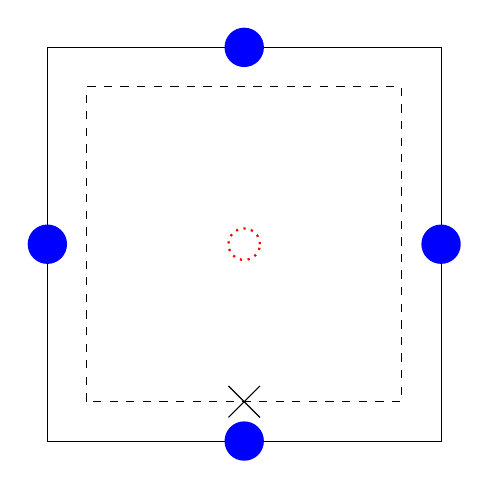
\begin{tikzpicture}

\draw (0,0) rectangle (5,5); % Outline of room

\draw[red,thick,dotted] (2.5,2.5) circle (0.2); % Phone location

\fill[blue!100!] (2.5, 0) circle (0.25); % Beacon location - Bottom
\fill[blue!100!] (5, 2.5) circle (0.25); % Beacon location - Right
\fill[blue!100!] (2.5, 5) circle (0.25); % Beacon location - Top
\fill[blue!100!] (0, 2.5) circle (0.25); % Beacon location - Left

% Walking path
\draw[dashed] (0.5,0.5) rectangle (4.5,4.5);

% Start / stop point of walking path
\draw (2.3,0.7) -- (2.7,0.3);
\draw (2.3,0.3) -- (2.7,0.7);

\end{tikzpicture}
  \caption{Illustration of room used for indoor location precision test. The full (blue) circles represent beacons, the dotted line is the walking path for the movement tests and the dotted center circle is the location of the phone for the stationary tests.}
  \label{fig:precisiontest:illustration}
\end{figure}

The setup consisted of four beacons, one on each wall, 
each using the recommended settings from Estimote \cite{estimote:settings}:
\begin{description}
  \item[Broadcasting Power:]{\num{4} dBm}
  \item[Advertising Interval:]{\SI{200}{\milli\second}}
  \item[Smart Power Mode:]{Enabled}
  \item[Basic Power Mode:]{Disabled}
\end{description}
The beacons run firmware version A3.2.0 and hardware version,
and the broadcasting scheme is the Estimote default scheme (\ie). 

For Room 3, the outdoor ``room'',
we attached the beacons to lampposts. 
We tested outside to see if the number of access points would have, and how much of, 
an impact on the accuracy. 
The ``room'' is illustrated in \Cref{fig:outdoortest}. 
The beacons in this room are slightly off-center (\SI{0.45}{\meter}), 
as we had to use the lampposts' locations. 

\begin{figure}[!htb]
  \centering
  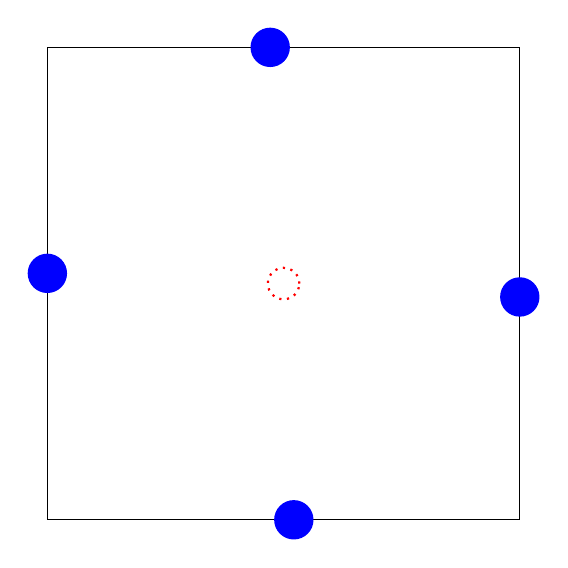
\begin{tikzpicture}

\draw (0,0) rectangle (6,6); % Outline of room
%
\draw[red,thick,dotted] (3,3) circle (0.2); % Phone location

\fill[blue!100!] (3.13, 0) circle (0.25); % Beacon location - Bottom
\fill[blue!100!] (6, 2.83) circle (0.25); % Beacon location - Right
\fill[blue!100!] (2.83, 6) circle (0.25); % Beacon location - Top
\fill[blue!100!] (0, 3.13) circle (0.25); % Beacon location - Left

\end{tikzpicture}
  \caption{Illustration of room used for Estimote accuracy outdoors, with little to no interference from WiFi access points. The full (blue) circles represent beacons, and the dotted center circle is the location of the phone (stationary test).}
  \label{fig:outdoortest}
\end{figure}

Room 4 is a seminar room. 
The setup for Room 4 for the stationary tests,
were exactly the same as the Room 1 and 2. 
We also did movement tests in this room, 
where the user walked around near the walls as done in Room 1 and 2. 
We did, however, also test movement where the user walked in a \emph{bowtie},
illustrated by \Cref{fig:bowtie4beacons}. 
We did this to see if we it would have any effect if we did not walk near the beacons all the time. 
We also tried to perform tests with \num{8} beacons in this room, 
illustrated by \Cref{fig:bowtie8beacons}. 

\begin{figure}[!htb]
  \begin{minipage}[b]{0.45\textwidth}
    \centering
    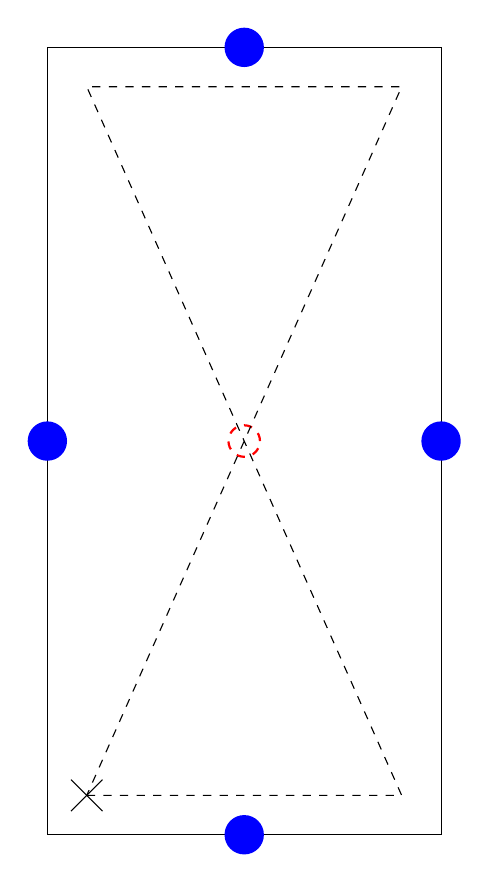
\begin{tikzpicture}

\draw (0,0) rectangle (5,10); % Outline of room

\draw[red,thick,dashed] (2.5,5) circle (0.2); % Phone location

\fill[blue!100!] (2.5, 0) circle (0.25); % Beacon location - Bottom
\fill[blue!100!] (5, 5) circle (0.25); % Beacon location - Right
\fill[blue!100!] (2.5, 10) circle (0.25); % Beacon location - Top
\fill[blue!100!] (0, 5) circle (0.25); % Beacon location - Left

% Walking path
\draw[dashed] (0.5,0.5) -- (4.5,0.5) -- (0.5, 9.5) -- (4.5, 9.5) -- cycle;

% Start / stop point of walking path
\draw (0.3,0.7) -- (0.7,0.3);
\draw (0.3,0.3) -- (0.7,0.7);

\end{tikzpicture}
    \caption{Room 4 bowtie setup using four beacons.}
    \label{fig:bowtie4beacons}
  \end{minipage}\hfill
  \begin{minipage}[b]{0.45\textwidth}
    \centering
    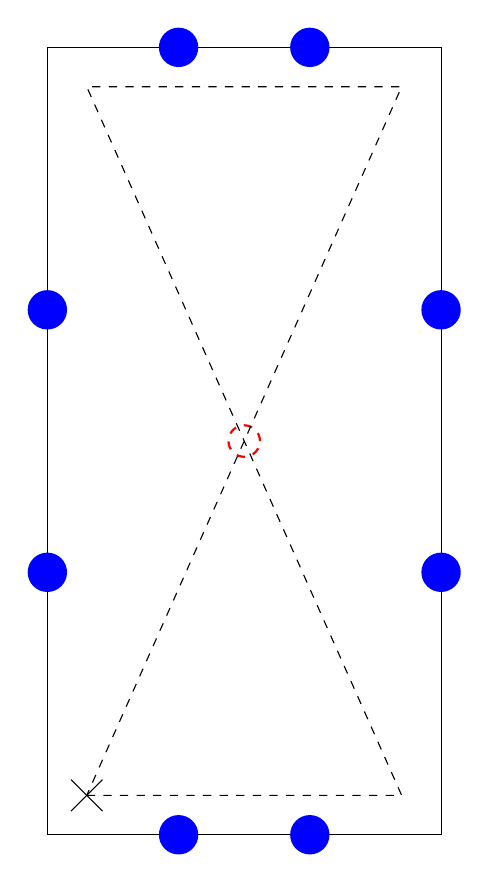
\begin{tikzpicture}

\draw (0,0) rectangle (5,10); % Outline of room

\draw[red,thick,dashed] (2.5,5) circle (0.2); % Phone location

\fill[blue!100!] (1.6667, 0) circle (0.25); % Beacon location - Bottom Left
\fill[blue!100!] (3.3334, 0) circle (0.25); % Beacon location - Bottom Right
\fill[blue!100!] (5, 6.6666) circle (0.25); % Beacon location - Right Top
\fill[blue!100!] (5, 3.3333) circle (0.25); % Beacon location - Right Bottom
\fill[blue!100!] (1.6667, 10) circle (0.25); % Beacon location - Top Left
\fill[blue!100!] (3.3334, 10) circle (0.25); % Beacon location - Top Right
\fill[blue!100!] (0, 6.6666) circle (0.25); % Beacon location - Left Top
\fill[blue!100!] (0, 3.3333) circle (0.25); % Beacon location - Left Bottom


% Walking path
\draw[dashed] (0.5,0.5) -- (4.5,0.5) -- (0.5, 9.5) -- (4.5, 9.5) -- cycle;

% Start / stop point of walking path
\draw (0.3,0.7) -- (0.7,0.3);
\draw (0.3,0.3) -- (0.7,0.7);

\end{tikzpicture}
    \caption{Room 4 bowtie setup using eight beacons.}
    \label{fig:bowtie8beacons}
  \end{minipage}
\end{figure}

\Cref{table:precisiontest:roomsize} shows the test setups from these rooms.
In \Cref{sec:settings}, we change some of the settings to determine if they have any effect.

\begin{table}[!htb]
  \centering
  \begin{tabular}{l| l l c c}
    Room   & Phone Position & Duration 	       & Test Count & \# of Beacons \\ \hline
    Room 1 & Center         & \SI{1}{\minute}  & 4          & 4 \\ 
    Room 1 & Center         & \SI{2}{\minute}  & 1          & 4 \\ 
    Room 1 & Moving         & NA               & 3          & 4 \\
    Room 2 & Center         & \SI{1}{\minute}  & 3          & 4 \\ 
    Room 2 & Center         & \SI{2}{\minute}  & 1          & 4 \\
    Room 2 & Moving         & NA               & 3          & 4 \\ 
    Room 3 & Center         & \SI{1}{\minute}  & 3          & 4 \\ 
    Room 4 & Center         & \SI{1}{\minute}  & 3          & 4 \\ 
    Room 4 & Center         & \SI{1}{\minute}  & 3          & 8 \\ 
    Room 4 & Moving         & NA               & 3          & 4 \\
    Room 4 & Moving         & NA               & 3          & 8 \\
    Room 4 & Moving-Bowtie  & NA               & 3          & 4 \\
    Room 4 & Moving-Bowtie  & NA               & 3          & 8 \\
  \end{tabular}
  \caption{Tests conducted with varying room size and recommended beacon configuration.}
  \label{table:precisiontest:roomsize}
\end{table}

\subsection{Stationary Accuracy}
This section contains the results from measuring the accuracy of the tests, 
where we have placed a phone and logged the locations. 
\Cref{fig:room3:1:4:c,fig:room4:1:4:c,fig:room4:1:4:2.8,fig:room4:1:8:c} shows selected results as heatmaps. 
In these heatmaps, the heat, or intensity, 
shows the number of coordinates measured at that coordinate. 
Located to the right of each of these figures, 
is a graph showing the distance error from that test. 
We use the Euclidean distance to calculate the distance error between the location of the phone, 
and each of the locations reported by the app:
\begin{equation}
 \var{distanceError(phone, app)} = \sqrt{(\var{phone.x} - \var{app.x})^2 + (\var{phone.y} - \var{app.y})^2}
\end{equation}

%HEATMAPS AND MEAN ERRORS
\newcommand{\graphspace}{\vspace{0.08cm}}
\begin{figure}[!htb]
  \begin{minipage}[b]{0.5\textwidth}
    \centering
    \includegraphics{\heatmap{32}}
    \graphspace
    \caption{Room 3, \SI{1}{\minute}, 4 beacons, centered}
    \label{fig:room3:1:4:c}
  \end{minipage}\hfill
  \begin{minipage}[b]{0.45\textwidth}
%    \centering
    \meanerror{32-outside-1218-1790x1790-1min.csv}{11}
    \caption{Distance error from \Cref{fig:room3:1:4:c}}
    \label{fig:distance:room3:1:4:c}
  \end{minipage}
\end{figure}

\begin{figure}[!htb]
  \begin{minipage}[b]{0.5\textwidth}
    \centering
    \includegraphics{\heatmap{36}}
    \graphspace
    \caption{Room 4, \SI{1}{\minute}, 4 beacons, centered}
    \label{fig:room4:1:4:c}
  \end{minipage}\hfill
  \begin{minipage}[b]{0.45\textwidth}
    \centering
    \meanerror{36-1911-1027-490x995-1min.csv}{4}
    \caption{Distance error from \Cref{fig:room4:1:4:c}}
    \label{fig:distance:room4:1:4:c}
  \end{minipage}
\end{figure}

\begin{figure}[!htb]
  \begin{minipage}[b]{0.5\textwidth}
    \centering
    \includegraphics{\heatmap{43}}
    \graphspace
    \caption{Room 4, \SI{1}{\minute}, 4 beacons, at (2,8)}
    \label{fig:room4:1:4:2.8}
  \end{minipage}\hfill
  \begin{minipage}[b]{0.45\textwidth}
    \centering
    \meanerror{43-1911-1106-490x995-1min-at-8.2.csv}{3}
    \caption{Distance error from \Cref{fig:room4:1:4:2.8}}
    \label{fig:distance:room4:1:4:2.8}
  \end{minipage}
\end{figure}

\begin{figure}[!htb]
  \begin{minipage}[b]{0.5\textwidth}
    \centering
    \includegraphics{\heatmap{51}}
    \graphspace
    \caption{Room 4, \SI{1}{\minute}, 8 beacons, centered}
    \label{fig:room4:1:8:c}
  \end{minipage}\hfill
  \begin{minipage}[b]{0.45\textwidth}
    \centering
    \meanerror{51-1911-1137-490x995-1min-8-beacons.csv}{4}
    \caption{Distance error from \Cref{fig:room4:1:8:c}}
    \label{fig:distance:room4:1:8:c}
  \end{minipage}
\end{figure}

The heatmaps shows that none of the results are very accurate. 
However, we do see some consistency in the data, in the form of clusters. 
This is primary seen in \Cref{fig:room3:1:4:c,fig:room4:1:4:2.8}. 
We do see some clustering in \Cref{fig:room4:1:4:c}. 
We expect the reason why the data is spread out like that, 
is a combination of the fact that the phone is centered, \ie not near any beacons,
and that we are near WiFi access points with the same frequency. 
We see a similar tendency in in \Cref{fig:room4:1:8:c}, 
but we expect that the increased spreading here is due to interference from using more beacons. 

The distance error graphs supports the statement that none of the results are very accurate. 
It is clearly worst in the outside test, shown by \Cref{fig:distance:room3:1:4:c}. 
\Cref{fig:distance:room4:1:4:2.8,fig:distance:room4:1:4:c} show some decent results. 
\Cref{fig:distance:room4:1:4:2.8}, where the phone is not centered, 
is the best result we get. 
An interesting result is seen by \Cref{fig:room4:1:8:c},
where it seems that the number of beacons, 
makes the measurements fluctuate. 

\Cref{table:meanerrorresults} shows the \emph{mean} distance error of all the stationary tests. 

\begin{table}[!htb]
  \centering
  \begin{tabular}{l|l c c}
    Room   & Position   & \# of beacons & Mean error \\ \hline
    Room 1 & Centered   & 4             & \SI{1.78}{\meter} \\
    Room 2 & Centered   & 4             & \SI{2.96}{\meter} \\
    Room 3 & Centered   & 4             & \SI{7.31}{\meter} \\
    Room 4 & Centered   & 4             & \SI{1.94}{\meter} \\
    Room 4 & At $(2,8)$ & 4             & \SI{1.22}{\meter} \\
    Room 4 & Centered   & 8             & \SI{3.02}{\meter} \\ \hline
    Total  &            &               & \SI{2.92}{\meter}
  \end{tabular}
  \caption{Mean error of all stationary tests with Estimote recommended settings. Some rooms have more test results than others. See \Cref{table:rooms}.}
  \label{table:meanerrorresults}
\end{table}

Based on this table, we can conclude the following:
\begin{itemize}
  \item The distance error increases as we increase the distance to the beacons
  \item Adding more beacons results in worse accuracy
\end{itemize}

Increasing the distance to the beacons, results in weaker signals from the beacons. 
It is thus expectable that the accuracy is worse further away from the beacons. 

Regarding the worse accuracy with more beacons, 
we have two theories to why.
The first theory is that the Estimote SDK only uses a subset of beacons, \eg only \num{4}, for accuracy. 
The reasoning behind this theory is that in \Cref{fig:distance:room4:1:8:c}, 
we consistent change between \SI{3.5}{\meter} and \SI{2.5}{\meter}, 
where from the tests with \num{4} (\Cref{fig:distance:room3:1:4:c,fig:distance:room4:1:4:c,fig:distance:room4:1:4:2.8}) beacons, 
we see a convergence after the first \num{50} measurements.
The change could be a result of Estimote changing from two sets of \num{4} beacons, 
where the \SI{3.5}{\meter} results are from one set, 
and the \SI{2.5}{\meter} results are from the other set. 
Estimote has not provided any documentation about how many beacons is used to get the location using the SDK, 
nor are we able to see this from the SDK. 

The other theory is that the beacons interfere with each other. 
With \num{8} beacons in a $5 \times 10$ meter room, 
it is possible that the signals interfere with each other, 
when the beacons are placed near to each other. 
In Estimote's guide for beacon placement \cite{SIGNALBLEED}, 
they write:
\begin{quote}
  ``If you’re using many beacon regions in close proximity to each other, it’s likely that you will experience \emph{signal bleed}: beacons from one region being detected in the other.''
\end{quote}
So it is possible that the signals we read from a beacon is from another beacon,
and thus we get a wrong reading.  

\FloatBarrier
\subsection{Moving Accuracy}
In this section we measure the accuracy of the Estimote beacons,
while the phone is in motion. 
We walk around in a given path, 
as described by \Cref{sec:setup}.
\Cref{fig:room1:4:m,fig:room2:4:m,fig:room4:4:m} shows selected heatmaps of walking near the walls, 
where \Cref{fig:room4:4:b,fig:room4:8:b} shows selected heatmaps of walking in a bowtie pattern.
%HEATMAPS
\begin{figure}[!htb]
  \begin{minipage}{0.48\textwidth}
    \centering
    \includegraphics[width=\textwidth]{\heatmap{08}}
    \caption{Room 1, 4 beacons, moving}
    \label{fig:room1:4:m}
  \end{minipage}\hfill
  \begin{minipage}{0.48\textwidth}
    \centering
    \includegraphics[width=\textwidth]{\heatmap{14}}
    \caption{Room 2, 4 beacons, moving}
    \label{fig:room2:4:m}
  \end{minipage}
\end{figure}
\begin{figure}[!htb]
  \centering
  \includegraphics[width=0.48\textwidth]{\heatmap{37}}
  \caption{Room 4, 4 beacons, moving}
  \label{fig:room4:4:m}
\end{figure}

\Cref{fig:room1:4:m,fig:room2:4:m} shows that the coordinates we get, 
were relatively close to where we walked, 
but had trouble near the corners, \ie further away from the beacons. 
\Cref{fig:room4:4:m} shows poor results. 
The main difference between rooms 1 and 2 and Room 4,
besides the size,  
is that Room 4 has actual walls, 
instead of the simulated walls. 
As walls can bounce radio waves from the beacons,
this is likely the reason why the results from Room 4 are worse. 

\begin{figure}[!htb]
  \begin{minipage}{0.48\textwidth}
    \centering
    \includegraphics[width=\textwidth]{\heatmap{40}}
    \caption{Room 4, 4 beacons, bowtie}
    \label{fig:room4:4:b}
  \end{minipage}\hfill
  \begin{minipage}{0.48\textwidth}
    \centering
    \includegraphics[width=\textwidth]{\heatmap{48}}
    \caption{Room 2, 8 beacons, bowtie}
    \label{fig:room4:8:b}
  \end{minipage}
\end{figure}
Like with \Cref{fig:room4:4:m}, \Cref{fig:room4:4:b,fig:room4:8:b} show poor results. 
This is likely due to walls, as with before, 
but also that we are now spending more time walking further away from beacons, 
than we did in \Cref{fig:room1:4:m,fig:room2:4:m}.

\subsection{Changing Settings}\label{sec:settings}
For this test the objective was to test the accuracy of the location system,
using different settings. 
We use Room 4 with 4 beacons for these tests. 
The tests conducted in this room, 
had the phone placed on a table in the center of the room, 
and logging position data for a duration of one minute.
This was done three times, 
and then the settings of the beacons were changed.

The different settings we tested are shown in \Cref{table:precisiontest:settings}.
Each result describes the mean error distance from \num{3} tests, 
each \num{1} minutes long.  

\begin{table}[!htb]
  \centering
  \begin{tabular}{c|c|c}
    Advertising Interval    & Broadcasting Power & Mean Error Distance \\ \hline
    \SI{200}{\milli\second} & \num{-20} dBm      & \SI{4.57}{\meter} \\ 
    \SI{200}{\milli\second} & \num{-12} dBm      & \SI{3.49}{\meter} \\ 
    \SI{200}{\milli\second} & \num{-4} dBm       & \SI{2.16}{\meter} \\ 
    \SI{200}{\milli\second} & \num{4} dBm        & \SI{2.81}{\meter} \\ 
    \SI{100}{\milli\second} & \num{4} dBm        & \SI{1.41}{\meter} \\ 
  \end{tabular}
  \caption{Tests conducted with varying settings on the beacons. Each result is from $3 \times 1$ minutes of measurement.}
  \label{table:precisiontest:settings}
\end{table}

The results from \Cref{table:precisiontest:settings} show that settings do have an impact on accuracy. However, the settings also have an impact on battery life. 
While changing from \SI{200}{\milli\second} to \SI{100}{\milli\second} almost increased accuracy by \perc{200},
it also increases the battery usage by \perc{200}.
Lower broadcasting powers such as \num{-20} dBm and \num{-12} dBm perform bad. 
This is because at such lower powers, 
the signal from the beacons might not have reached the phone, 
and the lack of data from these beacons is very likely to have worsened the accuracy.

Interestingly, \num{-4} dBm performed better than \num{4} dBm.
From \Cref{table:meanerrorresults}, we saw that more beacons worsened the accuracy. 
It is possible that a broadcasting power of \num{4} dBm,
creates more interferences, and thus worse results, than \num{-4} dBm. 
We do not, however, have enough data to properly conclude this. 

\subsection{Precision of Indoor Location Conclusion}
From our results, we can conclude that we cannot, 
in our settings, reach high indoor accuracy using Estimote beacons. 
They claim that the accuracy is \num{0.5}-\num{1} meters, 
but our best result is \num{1.22} meter, 
and our average accuracy is \num{2.92} meters. 

No tendencies are shown across the results. 
This make it very hard, if not impossible,
to compensate for inaccurate results.  

\subsubsection{Considerations}
All of our experiments in this section have been performed on a single device.
We cannot say if using a different phone would provide the same results.
The tests were performed on an iPhone 6 Plus running iOS 9.1.

Even though we have switched beacons between tests, 
so that we did not use the same ones every time, 
we have not tested if any of the beacons we have used are defect. 

The poor accuracy can also be from the SDK rather than the beacons. 
We have not tested whether we could obtain better results using other SDKs that are not provided by Estimote. 

Since all of our tests were performed at locations with considerable large number of WiFi access points as seen in \Cref{table:rooms},
the results could be affected by this. 
We did not test the locations in rooms with less access points, 
except for the outside room (Room 3), 
but where the size and settings of the room may have had too much effect on the results.